\documentclass[twoside,a4paper]{article} %Produces two pages (based on A4 paper size)
\usepackage{graphicx} % Required for inserting images
\usepackage[T1]{fontenc}
\usepackage[utf8]{inputenc}
\usepackage[czech]{babel}
\usepackage{hyperref}
\usepackage{xparse,nameref}
\usepackage{geometry}
\usepackage[autostyle=true,czech=quotes]{csquotes}
\usepackage{fancyhdr}
\usepackage[backend=biber, style=iso-numeric, alldates=iso,  sorting=nty]{biblatex} % bibliografie

\usepackage[table]{xcolor}
\usepackage{listings}
\usepackage{float}
\usepackage{algorithm2e}

 \lstset{
    language=C++,                    % Jazyk (C++)
    basicstyle=\ttfamily\footnotesize,% Základní styl písma (monospace)
    keywordstyle=\bfseries\color{blue},   % Klíčová slova (tučné a modré)
    stringstyle=\color{orange},       % Řetězce (oranžové)
    commentstyle=\itshape\color{green!50!black}, % Komentáře (kurzíva a tmavě zelené)
    numbers=left,                     % Číslování řádků vlevo
    numberstyle=\tiny\color{gray},    % Styl čísel řádků
    stepnumber=1,                     % Každý řádek bude očíslován
    numbersep=10pt,                   % Vzdálenost čísel od kódu
    backgroundcolor=\color{gray!10},  % Pozadí kódu (světle šedé)
    showspaces=false,                 % Nezobrazovat mezery
    showstringspaces=false,           % Nezobrazovat mezery v řetězcích
    tabsize=4,                        % Tabulátor = 4 mezery
    captionpos=b,                     % Popisek pod kódem
    breaklines=true,                  % Dlouhé řádky se budou zalamovat
    breakatwhitespace=true,           % Zalamování při mezeře
    frame=single,                     % Rámeček kolem kódu
    rulecolor=\color{black},          % Barva rámečku
    escapeinside={\%*}{*},            % Pro LaTeXové příkazy v kódu
    morekeywords={nullptr, uint32_t, uint64_t} % Další klíčová slova
}


 \geometry{
 a4paper,
 %total={170mm,257mm},
 %width = 170mm,
 left=20mm,
 top=30mm,
 bottom=35mm,
 right=30mm
 }

\title{Teorie programování \\ \large Určeno pro 4. ročník oboru Informatika a Řídící systémy
}
\author{Bc. Lukáš Horák}
\date{\today}

\makeatletter         
\def\@maketitle{\begin{center}

\includegraphics[width = 160mm]{images/logo.png}\\[8ex]
{\Huge \@title  }\\[4ex] 
{\Large  \@author}\\[4ex] 
{\Large rev. 1.0}\\[4ex]
\@date\\[20ex]

\includegraphics[width = 70mm]{images/c_logo.png}\\[25ex]
\end{center}}
\makeatother

\fancyhead{}
\pagestyle{fancy}
\fancyhf{}
\fancyhf[EHL]{PRG - Teorie}
\fancyhf[EFL]{\thepage}
\fancyhf[EFR]{Bc. Lukáš Horák}
\fancyhf[OFL]{Bc. Lukáš Horák}
\fancyhf[OFR]{\thepage}
\fancyhf[OHR]{PRG - Teorie}
\renewcommand{\headrulewidth}{0pt}
\thispagestyle{empty}

\begin{document}

\maketitle
\thispagestyle{empty}

\newpage

\tableofcontents
\listoffigures
\listoftables

\newpage

\section{Kompilace jazyka C a C++}
Jedna z nejzákladnějších znalostí každého programátora by měla být znalost procesu kompilace programovacího jazyka, který využívá. Na následujícím obrázku lze vidět proces kompilace programovacího jazyka C a C++ a následně si taktéž i rozebereme podrobně, z čeho se jednotlivé části kompilace skládají.

\subsection{Fáze překladu}
\begin{figure}[H]
    \centering
    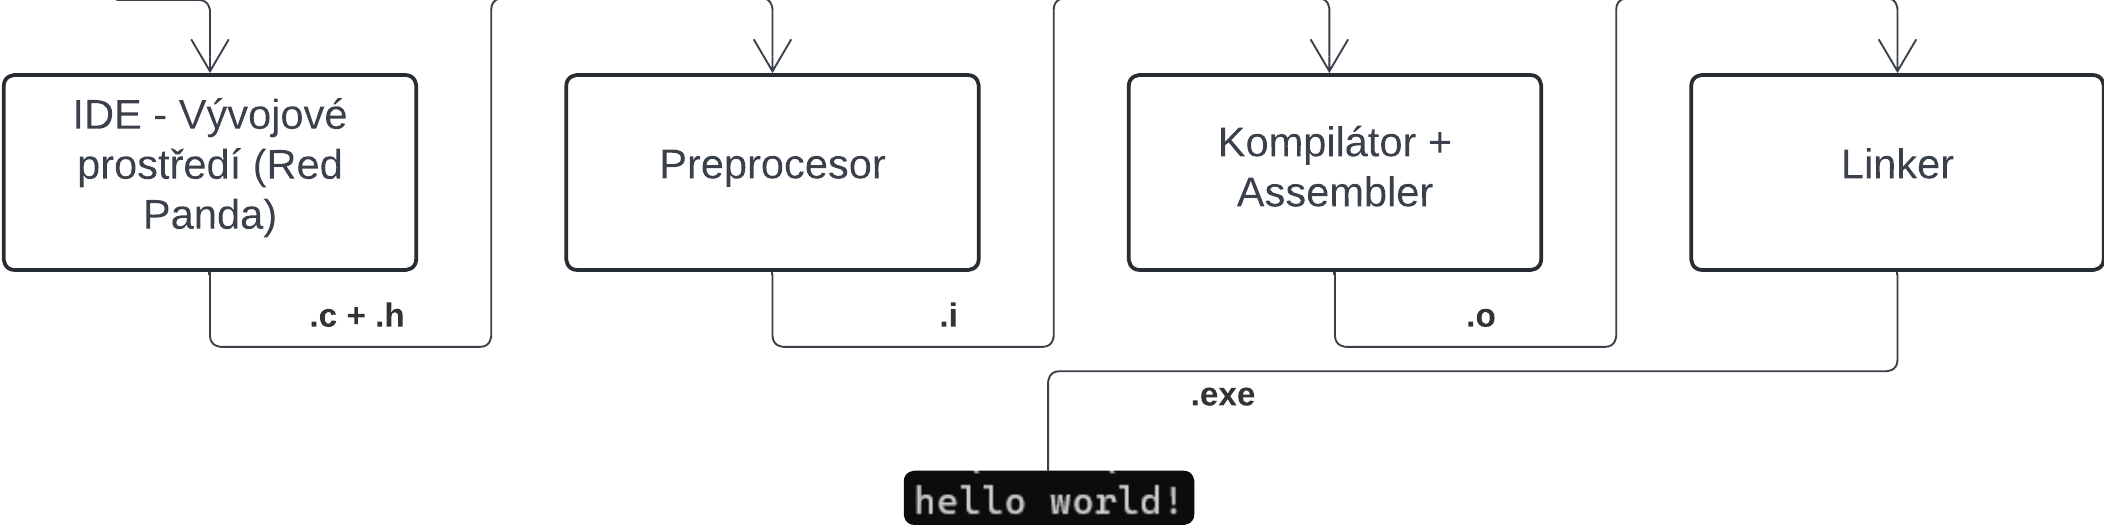
\includegraphics[width=0.95\linewidth]{images/compilation.png}
    \caption{Proces kompilace jazyka C}
    \label{fig:compilationOfC}
\end{figure}

\begin{itemize}
    \item \textbf{IDE} - IDE je vývojové prostředí, ve kterém programátor zapisuje zdrojový kód. Zdrojové kódy obsahují veškerou abstrakci i implementaci algoritmů sloužící pro správný chod programu. Výstupem z vývojového prostředí jsou soubory s příponami .c/.cpp/.h/.hpp a další.
    \item \textbf{Preprocesor} - Fáze preprocesoru nám slouží pro předzpracování již napsaného kódu a připravení jej pro následnou kompilaci. Preprocesor zkontroluje direktivy (tedy \#define, \#ifndef...) a nahrazuje je za funkční kód, popřípadě například podmíněných překladů (jako je \#ifdef) zkontroluje, zda-li je podmínka splněna, pokud podmínka splněná není, pak tuto danou část kódu preprocesor ze zdrojového kódu pro kompilátor odstraní. Výstupem jsou soubory s příponou .i
    \item \textbf{Kompilátor + Assembler} - Je část překladu, kdy se lidsky čitelný kód programovacího jazyka C a C++ převádí do formy assemblerovského kódu (jazyka strojových instrukcí), tento kód se převádí na kód strojový, který už není lidsky čitelný a je pro procesor čitelným. Každý soubor zdrojového kódu se převádí na samostatný objekt, což je také výstupem kompilátoru (soubory s příponou .o) a tyto soubory následně putují do linkeru.
    \item \textbf{Linker} - Linker je závěrečnou fází překladu a propojuje jednotlivé objekty do jednoho výsledného programu, popřípadě propojuje taktéž i více programu k sobě, pro jejich vzájemnou komunikaci. Soubory nalinkované přes linker mohou být buď statické nebo dynamické. Statické se ke zdrojovému kódu připojují hned během fáze překladu. Dynamické mají pouze odkaz a musejí se vyskytovat v systému během spouštění výsledného programu. Výhodou může být možná upravitelnost těchto dynamicky nalinkovaných knihoven, avšak nese to i riziko tzv. injectování kódu, tedy hrozbě, kdy útočník může nahradit kód dynamicky linkované knihovny za kód škodlivý, který je následně spuštěn s programem. Výsledkem linkeru je .exe soubor, který nazýváme taktéž jako binárka. Je to již spustitelný přeložený program.
\end{itemize}


\subsection{Jednoprůchodový překladač}
Za důležitou zmínku stojí taktéž i to, že kompilace programovacího jazyka C využívá jednoprůchodového překladače. To znamená že se program kompiluje takzvaně shora-dolů jedním průchodem. Kompilátor během tohoto jednoho průchodu ověřuje existenci veškerých proměnných a funkcí, které jsou během programu vyvolávány nebo používány. V případě zjištění chyby je kompilace přerušena a uživateli se zobrazí chybová hláška z fáze překladu odkazující na danou chybu. 

Pokud tedy program narazí během tohoto průchodu například na volanou funkci, kterou však během svého průchodu nezastihl, je vyvolána chyba o volání neexistující funkce ačkoliv se funkce ve zdrojovém kódu nachází, ale později, v takovém případě musíme před příkaz volající danou funkci vložit předpis dané funkce, nebo celou funkci včetně implementace. Příklad uveden níže.

\lstinputlisting[language=C]{codes/comp0.c}

Chybová hláška: [Warning]  implicit declaration of function 'soucet' [-Wimplicit-function-declaration]

Správné řešení:
\lstinputlisting[language=C]{codes/comp1.c}

\section{Datové typy a operátory jazyka C}
\subsection{Datové typy}
Programovací jazyk C rozpoznává několik datových typů, které nám určují typ proměnné. Mezi základní rozpoznáváme jako \textbf{neurčitý, celočíselné, reálné a znakové}. 

Příklady jednotlivých datových typů:
\begin{itemize}
    \item Neurčité:
    \begin{itemize}
        \item void
    \end{itemize}
    \item Celočíselné:
    \begin{itemize}
        \item char (8 bitů), short(16 bitů/WORD), long (64bitů), int (32bitů)
    \end{itemize}
    \item Reálné:
    \begin{itemize}
        \item float (32bitů), double(64bitů), long double(80 bitů)
    \end{itemize}
\end{itemize}

Rozpoznáváme kromě samotného typu taktéž i to, jestli je znaménkový nebo neznaménkový. To znamená, že rozlišujeme, zda-li číslo může být i záporné nebo jen kladné. Všechny datové typy, pokud neurčíme jinak, mají v základě nastavený datový typ znaménkový. Pokud chceme specifikovat, že se má jednat o neznaménkový, pak před typ musíme napsat klíčové slovo \textbf{unsigned}.

Příklad celočíselné proměnné \textbf{int} a \textbf{unsigned int}:
\begin{itemize}
    \item Oba tyto datové typy mají 32 bitů.
    \item První z nich má kladnou a zápornou část. Druhý jen kladnou.
    \item Datový typ \textbf{int} má interval čísel:
    \begin{equation}
        int \in \hspace{6px} <-2147483648;2147483647>  
    \end{equation}
    \item Datový typ \textbf{unsigned int} má interval čísel:
    \begin{equation}
        unsigned\_int \in \hspace{6px} <0;4294967295>
    \end{equation}
\end{itemize}

Zajímavostí programovacího jazyka C je ta, že rozdíl mezi znakem a celým číslem v jazyce rozdíl téměř není. Tam, kde se dá použít datový typ \textbf{integer} se dá taktéž použít i datový typ \textbf{char}. Zde je příklad při použití u větvení programovacího jazyka C pomocí switche.

\lstinputlisting[language=C]{codes/switch0.c}
\lstinputlisting[language=C]{codes/switch1.c}

V prvním příkladě můžeme vidět switch použitý s celočíselnou podmínkou. Naopak u druhého příkladu můžeme vidět použití se znaky, jenže u těchto znaků taktéž vidíme, že používáme čísla. Tato čísla pocházejí z ASCII tabulky znaků.

\begin{figure}[H]
    \centering
    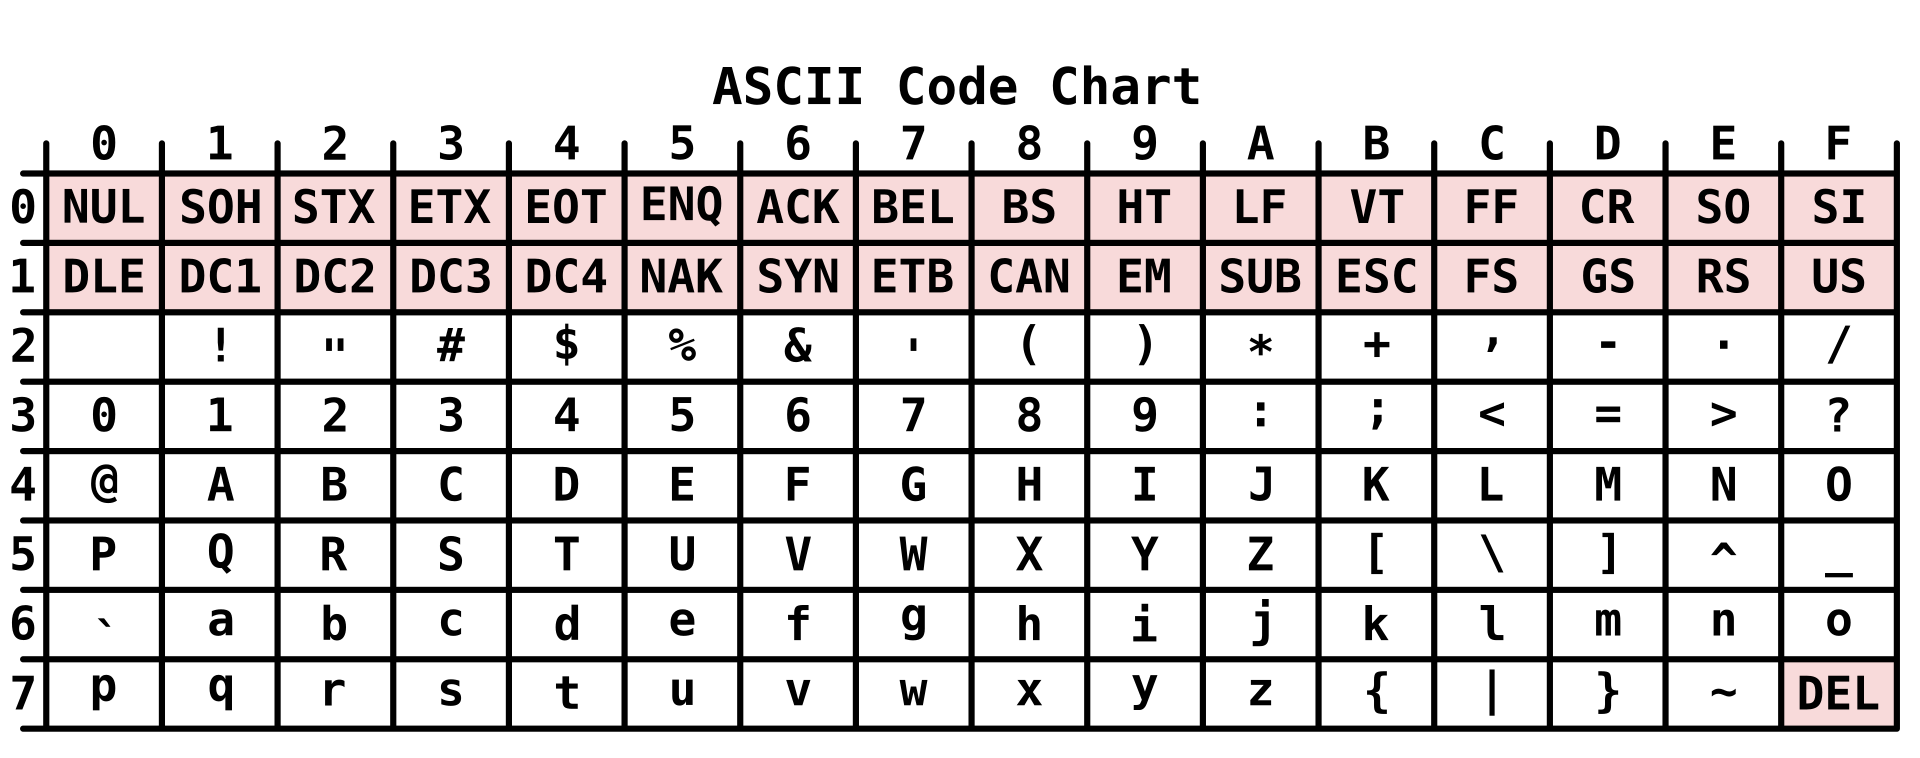
\includegraphics[width=0.7\linewidth]{images/ASCII.png}
    \caption{ASCII tabulka znaků}
    \label{fig:asciiTable}
\end{figure}

Pokud si například deklarujeme číslo se stejnou hodnotou, jako je tomu v ASCII tabulce, pak při výpisu pomocí printf jsme schopni vypsat toto celé číslo jako znak a opravdu bude odpovídat tomu stejnému znaku, jako bychom chtěli použít u typu char.

\subsection{Operátory}
Rozpoznáváme také několik typů operátorů jako jsou bitové, porovnávací (relační), inkrementační, dekrementační, aritmetické.

Příklady jednotlivých operátorů:
\begin{itemize}
    \item Bitové
    \begin{itemize}
        \item << >> bitový posun
        \item \& AND
        \item | OR
        \item \texttt{\^{}} XOR
        \item \textasciitilde Negace
    \end{itemize}
    \item Přiřazení
    \begin{itemize}
        \item += -= *= /=
        \item =
    \end{itemize}
    \item Relační a logické operátory
    \begin{itemize}
        \item < > >= <= == Relační operátory
        \item \&\& || ! Logické operátory
    \end{itemize}
    \item Inkrementace a dekrementace
    \begin{itemize}
        \item ++ 
        \item --
    \end{itemize}
    \item Aritmetické
    \begin{itemize}
        \item Unární operátory
        \begin{itemize}
            \item + - * / \% (modulo/zbytek po dělení)
        \end{itemize}
    \end{itemize}
\end{itemize}

\textbf{Poznámka \#1:} U inkrementace a dekrementace záleží na pořadí. Tedy jestli máme například proměnnou \textbf{x} a ta má operátor x++ nebo ++x. Standardně v kódu to změnu neudělá, avšak například u výpisu ano. Příklad:

\lstinputlisting[language=C]{codes/incDec.c}

Na výstupu výše zmíněného kódu bude výpis u proměnné \textbf{a} roven \textbf{0}, jelikož nejdříve to vypíše obsah dané proměnné a až následně proměnnou inkrementuje. Naopak je tomu u příkladu s proměnnou \textbf{b}, kde se nejdříve proměnná inkrementuje a až následně vypíše. Výstupem tedy bude hodnota rovna \textbf{1}.

\textbf{Poznámka \#2:} U modula se dá dělit pouze dvě celočíselné hodnoty, nemůžeme použít na čísla s plovoucí desetinnou čárkou nebo jakékoliv reálné číslo.

\section{Logické brány}
Tato část pojednává o branách, které bychom již měli znát z číslicové techniky a vyzkoušíme si je uvést na příkladech z programovacího jazyka C/C++. V Tabulce uvedené níže můžeme vidět příklad takových bran na dvou proměnných \textbf{a} a \textbf{b}. Konkrétně si zde budeme rozebírat pouze ty brány, které používáme i základně v programovacím jazyce C/C++.


\begin{table}[H]
    \centering
    \begin{tabular}{|c|c||c|c|c|c|c|}
      \rowcolor{yellow}\hline  a & b & a | b & a \& b & a \texttt{\^{}} b & \textasciitilde a & \textasciitilde b\\
        \hline 0 & 0 & 0 &  0& 0 &  1&1 \\
         \hline 0 & 1 & 1 &  0& 1 & 1 &0 \\
         \hline 1&  0&  1&  0&  1& 0 & 1\\
         \hline 1&  1&  1& 1 &  0& 0 & 0\\ \hline
    \end{tabular}
    \caption{Příklady logických bran}
    \label{tab:logicGates}
\end{table}

Uveďme si příklad výsledku dvou proměnných, nad kterými provedeme jednotlivé bitové operace a jaké budou jejich výsledky:

\lstinputlisting[language=C]{codes/logicGates.c}

Výstup z tohoto programu je následující:

\begin{figure}[H]
    \centering
    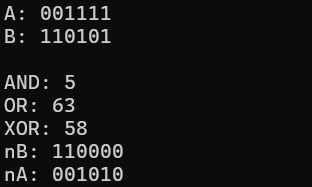
\includegraphics[width=0.4\linewidth]{images/logicGatesOutput.png}
    \caption{Výstup programu pro logické brány}
    \label{fig:placeholder}
\end{figure}

Je nutné nezapomínat na to, že pokud budeme používat bitové operace například v podmínce nějaké smyčky nebo v podmíněném větvení typu if nebo switch, je potřeba si uvědomit, že podmínka je vždycky \textbf{pravdivá} pokud je číslo nenulové. Pokud je hodnota rovna nule, pak je podmínka vyhodnocena jako \textbf{nepravdivá}.

\section{Obecná terminologie programování}
\subsection{Proměnné}
\subsection{Funkce}


\newpage

\newpage
\addcontentsline{toc}{section}{Reference}
\printbibliography
\nocite{*}

\end{document}
